\section{Pulling and inserting a plug}
	\label{sec:plug}
	
	\subsection{Outline of the plug task}
	
		One of the surprise tasks at the DRC consisted of pulling out a plug
		from one socket and putting it back into another socket, in a set-up like the one shown in
		\figurename~\ref{fig:Sockets-Plug}.
		The separation between both sockets was not known in advance, neither the height at which
		they were placed.
		Only the shape and size of the plug and the shape of the sockets (not their dimensions)
		were known in advance.
		
		\begin{figure}[t]
			\centering
			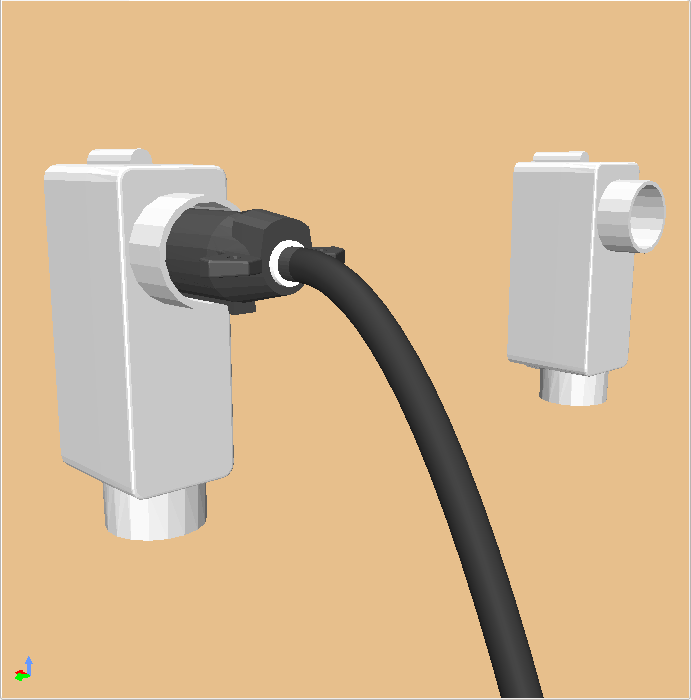
\includegraphics[height = 3.25cm]{img/Sockets-Plug}
			\caption{Plug Task. The robot must pull out the plug from one socket and insert it into the other.}
			\label{fig:Sockets-Plug}
		\end{figure}
		
		To carry out this task, we can consider its execution as divided into the following phases:
		%
		\begin{enumerate}
			\item Detection the socket and plug.
			\item Grasping the plug.
			\item Pulling and adjusting the plug.
			\item Inserting the plug.
		\end{enumerate}
	
	\subsection{Detection of the socket and plug}
		
		In order to perform this task it is first necessary to identify the plug and the socket where
		it is originally inserted, by placing the corresponding Manipulation Marker within the point cloud.
		The reason to identify both objects instead of just the plug is because almost half of it
		is not visible, as it is inside of the socket.
		As a consequence, the matching precision attained by aligning just the plug is lower than the one
		attained by aligning both objects.
		
		To do that we first detect all the planes in the scene, assuming that one of them will correspond
		to the wall where the sockets are installed.
		Then, given that the front face of the sockets is parallel to this wall, it is possible
		to calculate their orientation with respect to the robot.
		Having done this, one point belonging to the plug can be manually selected in order to compute
		an approximate initial position for the Manipulation Marker representing the socket and the plug.
		
		This initial position can be later refined, after the robot has arrived to a predetermined stance
		relative to the plug and after the point cloud has been adjusted by using one hand of the robot as
		a reference (given that its pose can be calculated from the internal sensors), as shown in
		\figurename~\ref{fig:SocketPlugMarker}.
		This is because the measured point cloud has some intrinsic noise, mainly caused as a result of
		the sunlight.
		
		\begin{figure}[b]
			\centering
			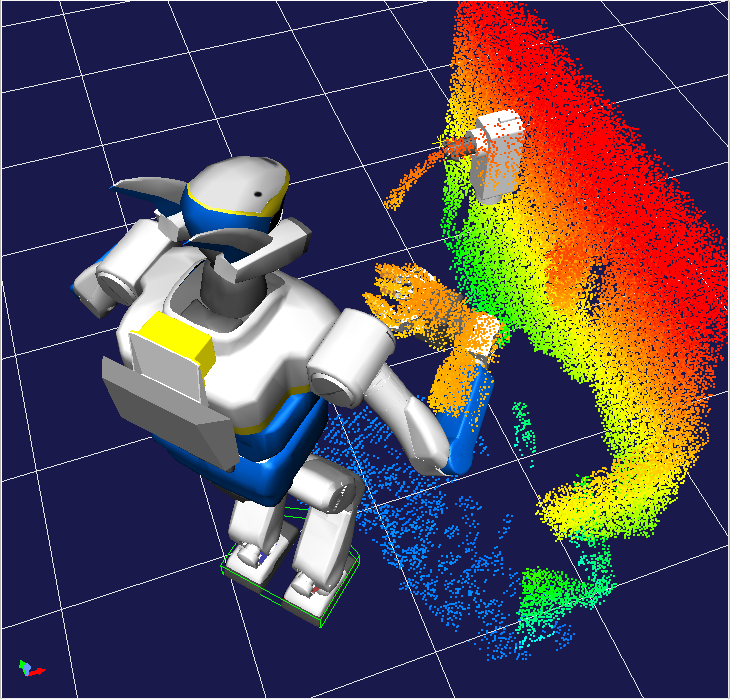
\includegraphics[height = 4.5cm]{img/SocketPlugMarker}
			\caption{Detection of the socket and the plug.}
			\label{fig:SocketPlugMarker}
		\end{figure}
		
	\subsection{Grasping the plug}
		
		Having detected an approximate pose for the socket, the robot first approaches the plug
		with one hand while aligning the camera installed at the other hand with the longitudinal axis
		of the plug.
		By doing this it is possible for the operator to make slight adjustments of the grasping hand
		by using the visual information provided by the hand camera.
		\figurename~\ref{fig:PreCloseHand} shows this configuration for the situation in which the plug
		is initially inserted into the left socket.
		Then, the robot uses its right hand to grasp the plug and the left hand for the camera.
		Were the plug initially inserted into the other socket, then the role for both hands would be
		reversed.
		
		\begin{figure}[t]
			\centering
			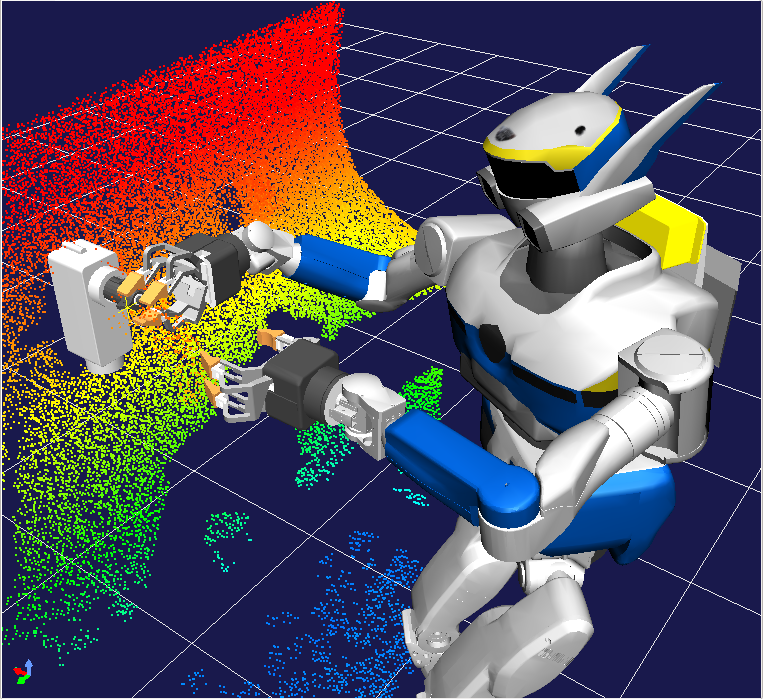
\includegraphics[height = 4.5cm]{img/PreCloseHand}
			\caption{Configuration of the robot before grasping the plug.}
			\label{fig:PreCloseHand}
		\end{figure}
		
		The size of the visible part of the plug is not that big compared to the hand of the robot,
		and because of that the allowable tolerance for grasping the plug is small.
		Then, it is required to grasp it at the point in which the hand also touches the socket.
		This can be done by translating the hand along the longitudinal axis of the plug until sensing
		30 N of force (enough for considering that it hits to the socket).
		This strategy is effective (when adjusted properly) as the grasp can be done every time at the
		desired point with enough precision even in the presence of uncertainties, as shown in the dynamical
		simulation depicted	in \figurename~\ref{fig:GraspPlug}.
		
		\begin{figure}[b]
			\centering
			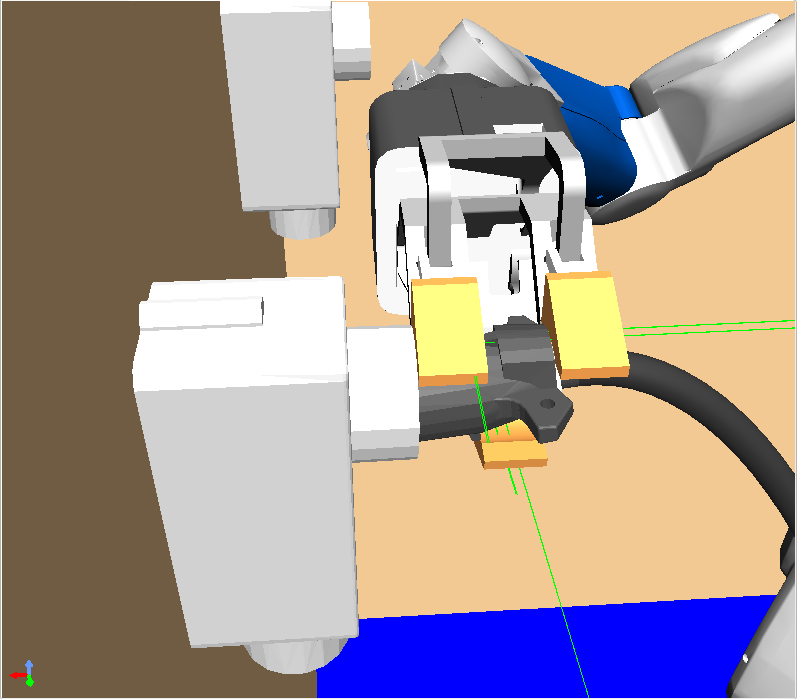
\includegraphics[height = 4.5cm]{img/GraspPlug}
			\caption{The plug being effectively grasped.}
			\label{fig:GraspPlug}
		\end{figure}
		
	\subsection{Pulling and adjusting the plug}
		
		After grasping the plug, the robot has to pull it.
		Due to the waist motion occurring during the stabilization of the robot, the pulling motion may not
		be performed exactly along the longitudinal axis of the plug, and this one may hit the inner walls
		of the socket while being pulled, modifying the planned relative pose between the plug and the
		grasping hand.
		
		For this reason, before inserting the plug into the other socket, the robot first brings the plug
		in front of its chest, takes an updated point cloud, and uses the camera placed at the head and
		at the other hand to look at the plug from two perpendicular directions, as seen in
		\figurename~\ref{fig:WatchPlug}.
		By using the point cloud, together with the visual information of both cameras, it is possible to
		fix the actual pose of the Manipulation Marker representing the plug to match the pose of
		the real one with respect to the hand.
		
		\begin{figure}[t]
			\centering
			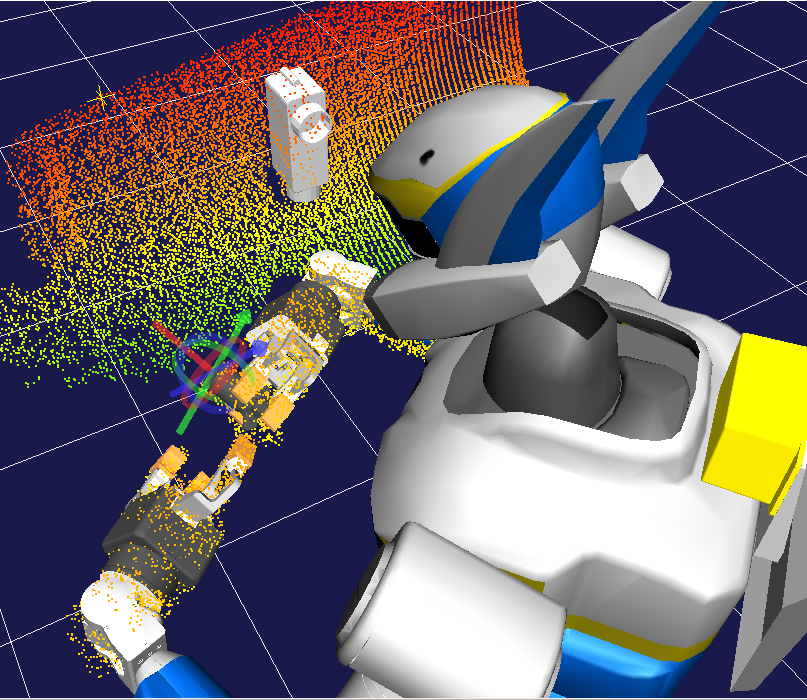
\includegraphics[height = 4.5cm]{img/WatchPlug}
			\caption{After pulling the plug its pose is adjusted.}
			\label{fig:WatchPlug}
		\end{figure}
		
	\subsection{Inserting the plug}
		
		Once this relative pose is known it is possible to align the plug with the destination socket,
		whose position can also be approximated by adjusting the corresponding marker within the point cloud.
		However, it is still worth to consider that this position may not be accurate enough,
		making it unfeasible to attempt an immediate insertion.
		Instead, the camera at the other hand can be used once again together with the camera at the head to
		look at the plug from two different points of view (as seen in \figurename~\ref{fig:InsertPlug}),
		in such a way that the operator can use this visual	information to slightly adjust the position of the
		plug before inserting it.
		
		\begin{figure}[b]
			\centering
			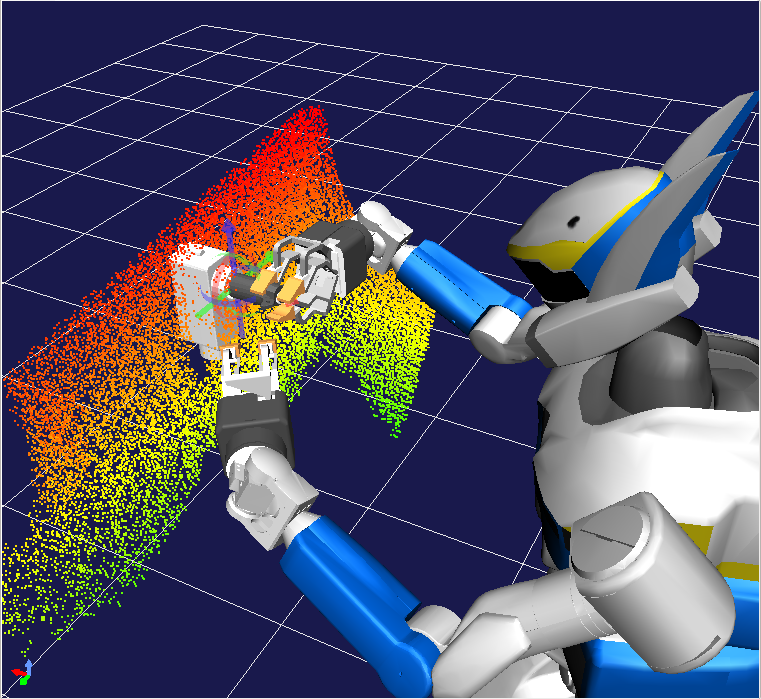
\includegraphics[height = 4.5cm]{img/InsertPlug}
			\caption{The plug is inserted by using visual feedback.}
			\label{fig:InsertPlug}
		\end{figure}
		
		Then, once the task is completed, the grasping hand opens and an updated point cloud is taken again,
		in order to plan the returning motion without hitting the cable of the plug.
		
	\subsection{Result at the DRC Finals}
		
		During the second day of the DRC Finals 2015 (June 6), HRP-2Kai was able to carry out
		the plug task within 16 minutes and 34 seconds, mainly because we were supervising every motion of the
		robot in order to prevent unexpected collisions, and also due to the blackouts that prevented us to make
		a faster identification of the plug in the point cloud.
		Even without knowing the disposition of the sockets within the field, HRP-2Kai was able to identify the
		plug, approach to it, grasp it, pull it and insert it into the other socket.
		Then, before returning to its home position, the hand of the robot grazed a portion of the plug not
		detected by the LRF and it fell down.
		However, the point corresponding to the task was granted, as the plug was inserted into the socket
		when the robot opened its hand.
		Some snapshots taken during the task at the DRC Finals are shown in \figurename~\ref{fig:plug-drc},
		together with the description of the current process in accordance with the explanation given before.
		
		\begin{figure}[t]
			\centering
			\subfloat[Identify plug in socket]
				{\label{fig:Plug_30_24_60} 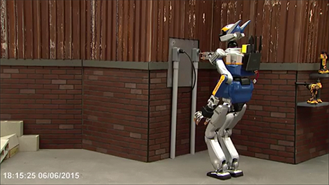
\includegraphics[height = 2cm]{img/Plug_30_24_60}}
			\subfloat[Adjust point cloud offset]
				{\label{fig:Plug_32_24_23} 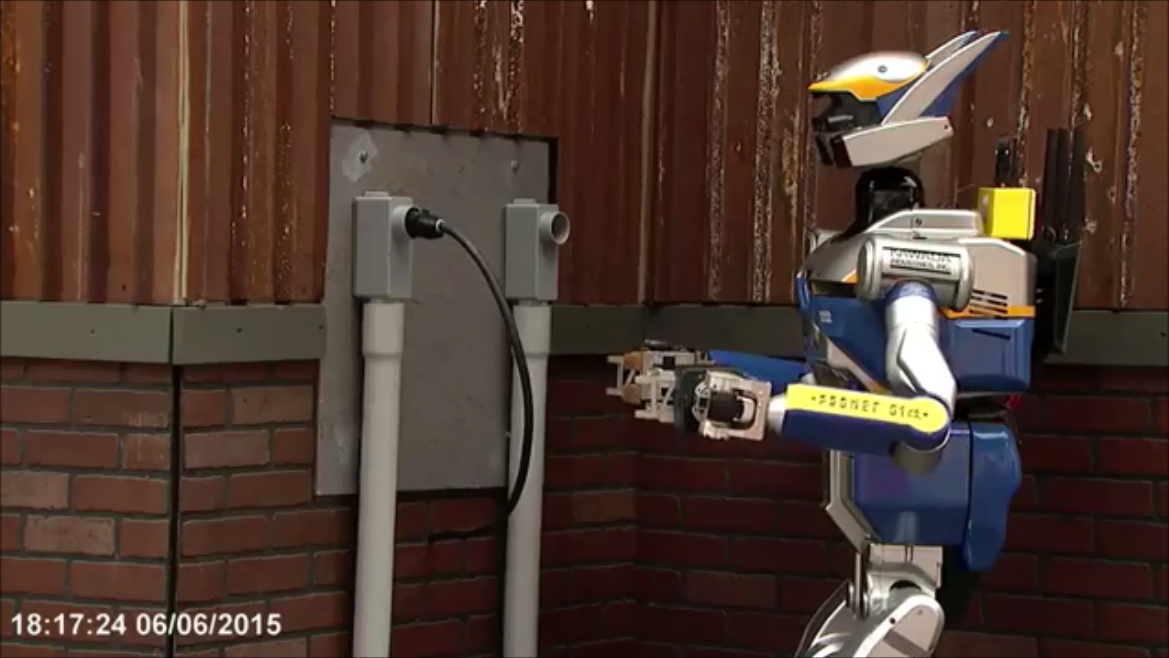
\includegraphics[height = 2cm]{img/Plug_32_24_23}}
			\\
			%
			\subfloat[Prepare for pre-grasping]
				{\label{fig:Plug_34_33_87} 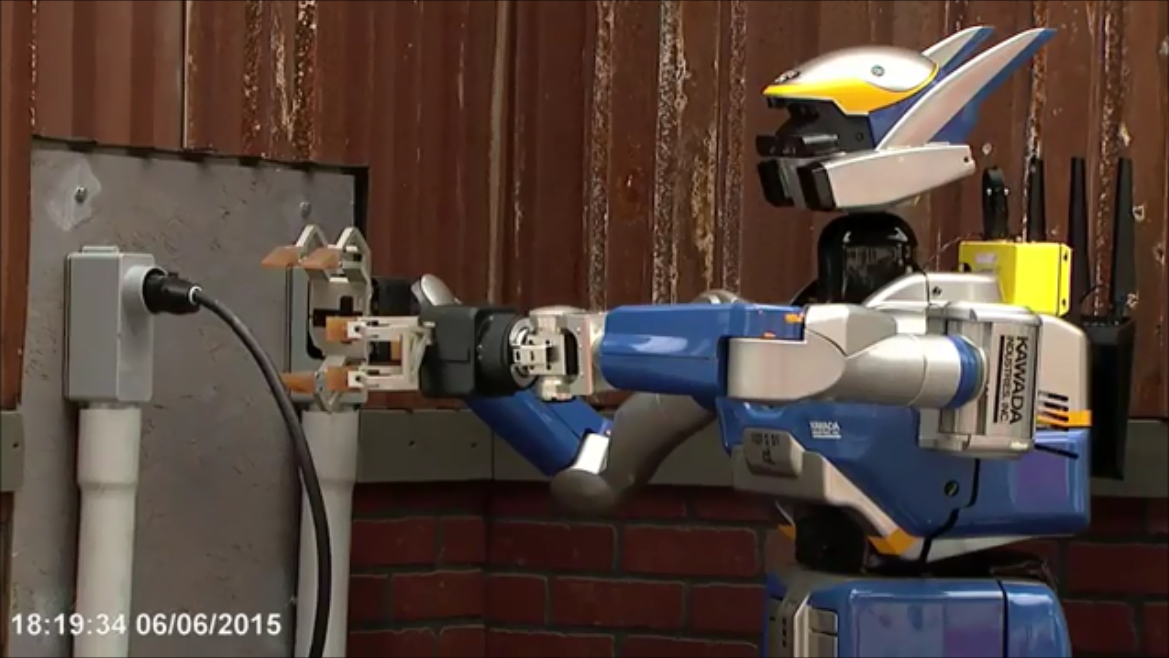
\includegraphics[height = 2cm]{img/Plug_34_33_87}}
			\subfloat[Align hand to grasp]
				{\label{fig:Plug_37_23_37} 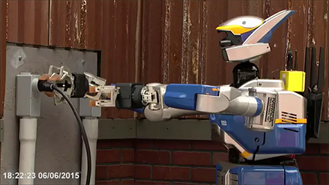
\includegraphics[height = 2cm]{img/Plug_37_23_37}}
			\\
			%
			\subfloat[Pull out the plug]
				{\label{fig:Plug_38_13_00} 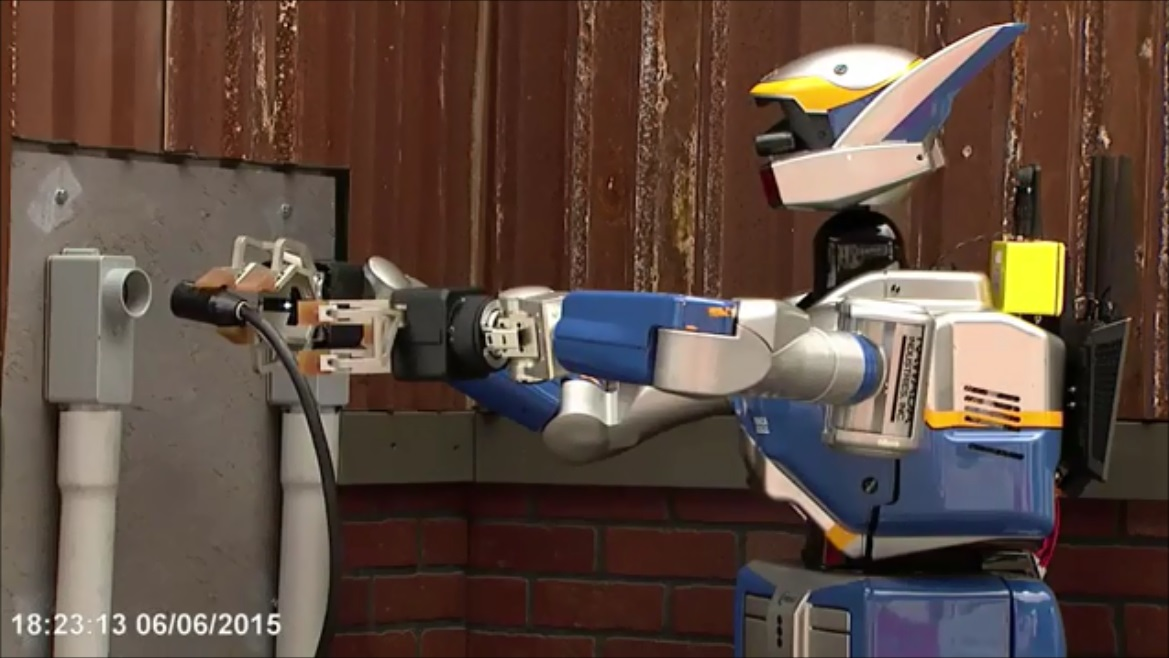
\includegraphics[height = 2cm]{img/Plug_38_13_00}}
			\subfloat[Identify plug in hand]
				{\label{fig:Plug_39_03_07} 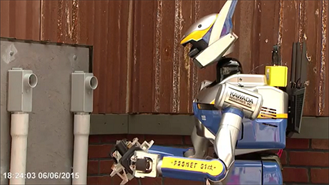
\includegraphics[height = 2cm]{img/Plug_39_03_07}}
			\\
			%
			\subfloat[Prepare for pre-insertion]
				{\label{fig:Plug_43_42_13} 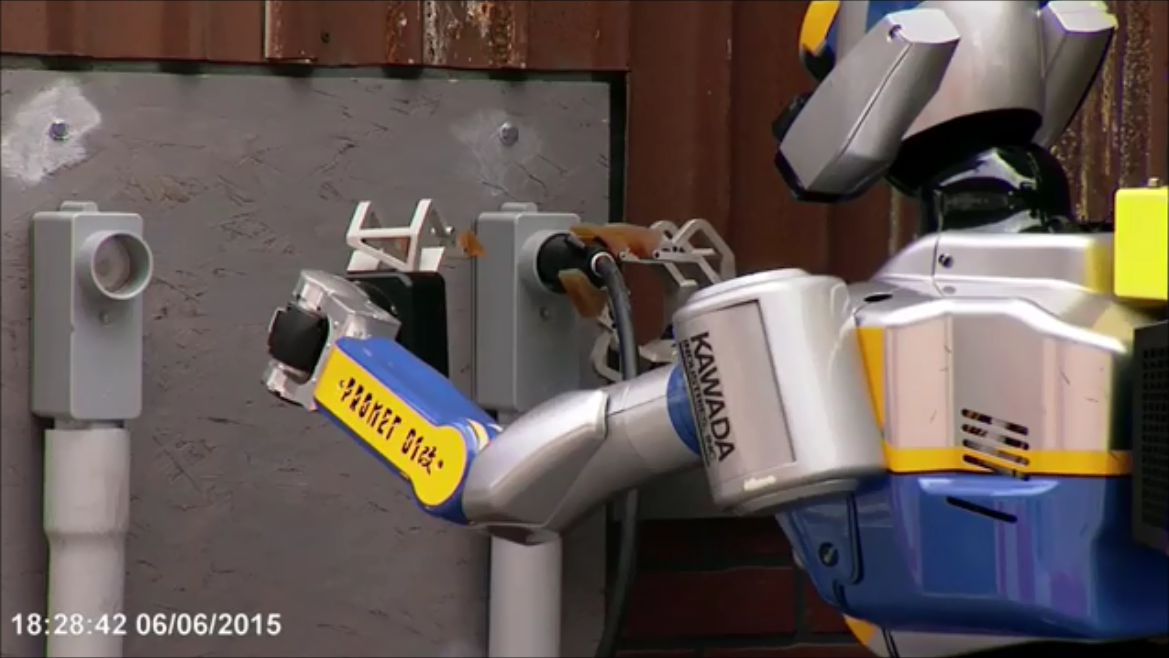
\includegraphics[height = 2cm]{img/Plug_43_42_13}}
			\subfloat[Plug is inserted]
				{\label{fig:Plug_44_51_93} 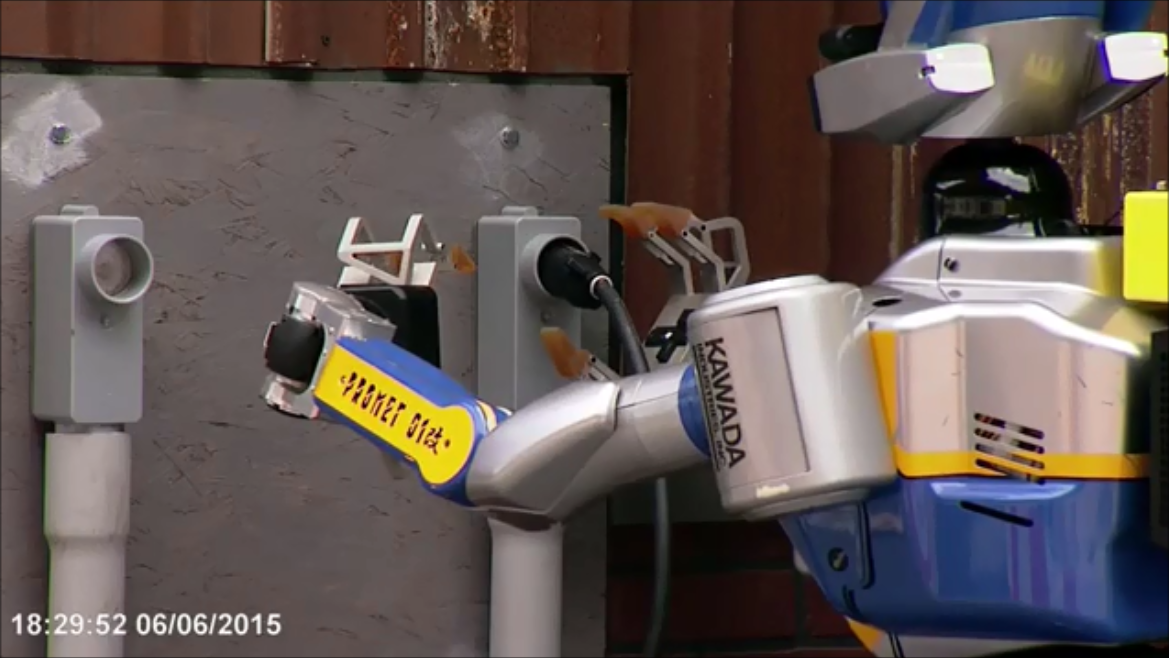
\includegraphics[height = 2cm]{img/Plug_44_51_93}}
			%
			\caption{Plug task at DRC Finals on June 6~\cite{DARPA}}
			\label{fig:plug-drc}
		\end{figure}
		
		Table~\ref{tab:teams} summarizes the performance obtained by the teams that were able to
		accomplish the plug task.
		For comparison effects, the following information is presented:
		the place obtained by each team during the competition, the time spent during the execution
		of the plug Task, the effective time of the task (by considering only the time in which the
		robot is moving) and the number of adjustments (intermittent correction motions) performed
		during the insertion of the plug.
		
		\begin{table}[t]
			%
			\caption{Teams that completed the plug task.}
			\label{tab:teams}
			\centering
			%
			\begin{tabular}{cccccc}
				\hline
				Team 					& Place	& Task	& Effective & Insertion	\\
											& 			& time	& time			& adjust.		\\
				\hline
				KAIST					& 1			& 11:01	& 2:18			& 14				\\
				IHMC Robotics	& 2			& 6:31	& 2:32			& 8					\\
				Tartan Rescue	& 3			& 18:33	& 3:21			& 17				\\
				NIMBRO Rescue	& 4			& 8:16	& 2:29			& 16				\\
				WPI-CMU				& 7			& 5:07	& 1:42			& 7					\\
				AIST-NEDO			& 10		& 16:34	& 1:34			& 3					\\
				\hline
			\end{tabular}
			%
		\end{table}